\documentclass[]{article}
\usepackage{lmodern}
\usepackage{amssymb,amsmath}
\usepackage{ifxetex,ifluatex}
\usepackage{fixltx2e} % provides \textsubscript
\ifnum 0\ifxetex 1\fi\ifluatex 1\fi=0 % if pdftex
  \usepackage[T1]{fontenc}
  \usepackage[utf8]{inputenc}
\else % if luatex or xelatex
  \ifxetex
    \usepackage{mathspec}
  \else
    \usepackage{fontspec}
  \fi
  \defaultfontfeatures{Ligatures=TeX,Scale=MatchLowercase}
\fi
% use upquote if available, for straight quotes in verbatim environments
\IfFileExists{upquote.sty}{\usepackage{upquote}}{}
% use microtype if available
\IfFileExists{microtype.sty}{%
\usepackage{microtype}
\UseMicrotypeSet[protrusion]{basicmath} % disable protrusion for tt fonts
}{}
\usepackage[margin=1in]{geometry}
\usepackage{hyperref}
\hypersetup{unicode=true,
            pdftitle={Laboratory Project - Final Report},
            pdfauthor={Henrique Costa, João Raimundo, João Rato, Pedro Gonçalves, Rodrigo Rente,},
            pdfborder={0 0 0},
            breaklinks=true}
\urlstyle{same}  % don't use monospace font for urls
\usepackage{color}
\usepackage{fancyvrb}
\newcommand{\VerbBar}{|}
\newcommand{\VERB}{\Verb[commandchars=\\\{\}]}
\DefineVerbatimEnvironment{Highlighting}{Verbatim}{commandchars=\\\{\}}
% Add ',fontsize=\small' for more characters per line
\usepackage{framed}
\definecolor{shadecolor}{RGB}{248,248,248}
\newenvironment{Shaded}{\begin{snugshade}}{\end{snugshade}}
\newcommand{\AlertTok}[1]{\textcolor[rgb]{0.94,0.16,0.16}{#1}}
\newcommand{\AnnotationTok}[1]{\textcolor[rgb]{0.56,0.35,0.01}{\textbf{\textit{#1}}}}
\newcommand{\AttributeTok}[1]{\textcolor[rgb]{0.77,0.63,0.00}{#1}}
\newcommand{\BaseNTok}[1]{\textcolor[rgb]{0.00,0.00,0.81}{#1}}
\newcommand{\BuiltInTok}[1]{#1}
\newcommand{\CharTok}[1]{\textcolor[rgb]{0.31,0.60,0.02}{#1}}
\newcommand{\CommentTok}[1]{\textcolor[rgb]{0.56,0.35,0.01}{\textit{#1}}}
\newcommand{\CommentVarTok}[1]{\textcolor[rgb]{0.56,0.35,0.01}{\textbf{\textit{#1}}}}
\newcommand{\ConstantTok}[1]{\textcolor[rgb]{0.00,0.00,0.00}{#1}}
\newcommand{\ControlFlowTok}[1]{\textcolor[rgb]{0.13,0.29,0.53}{\textbf{#1}}}
\newcommand{\DataTypeTok}[1]{\textcolor[rgb]{0.13,0.29,0.53}{#1}}
\newcommand{\DecValTok}[1]{\textcolor[rgb]{0.00,0.00,0.81}{#1}}
\newcommand{\DocumentationTok}[1]{\textcolor[rgb]{0.56,0.35,0.01}{\textbf{\textit{#1}}}}
\newcommand{\ErrorTok}[1]{\textcolor[rgb]{0.64,0.00,0.00}{\textbf{#1}}}
\newcommand{\ExtensionTok}[1]{#1}
\newcommand{\FloatTok}[1]{\textcolor[rgb]{0.00,0.00,0.81}{#1}}
\newcommand{\FunctionTok}[1]{\textcolor[rgb]{0.00,0.00,0.00}{#1}}
\newcommand{\ImportTok}[1]{#1}
\newcommand{\InformationTok}[1]{\textcolor[rgb]{0.56,0.35,0.01}{\textbf{\textit{#1}}}}
\newcommand{\KeywordTok}[1]{\textcolor[rgb]{0.13,0.29,0.53}{\textbf{#1}}}
\newcommand{\NormalTok}[1]{#1}
\newcommand{\OperatorTok}[1]{\textcolor[rgb]{0.81,0.36,0.00}{\textbf{#1}}}
\newcommand{\OtherTok}[1]{\textcolor[rgb]{0.56,0.35,0.01}{#1}}
\newcommand{\PreprocessorTok}[1]{\textcolor[rgb]{0.56,0.35,0.01}{\textit{#1}}}
\newcommand{\RegionMarkerTok}[1]{#1}
\newcommand{\SpecialCharTok}[1]{\textcolor[rgb]{0.00,0.00,0.00}{#1}}
\newcommand{\SpecialStringTok}[1]{\textcolor[rgb]{0.31,0.60,0.02}{#1}}
\newcommand{\StringTok}[1]{\textcolor[rgb]{0.31,0.60,0.02}{#1}}
\newcommand{\VariableTok}[1]{\textcolor[rgb]{0.00,0.00,0.00}{#1}}
\newcommand{\VerbatimStringTok}[1]{\textcolor[rgb]{0.31,0.60,0.02}{#1}}
\newcommand{\WarningTok}[1]{\textcolor[rgb]{0.56,0.35,0.01}{\textbf{\textit{#1}}}}
\usepackage{graphicx,grffile}
\makeatletter
\def\maxwidth{\ifdim\Gin@nat@width>\linewidth\linewidth\else\Gin@nat@width\fi}
\def\maxheight{\ifdim\Gin@nat@height>\textheight\textheight\else\Gin@nat@height\fi}
\makeatother
% Scale images if necessary, so that they will not overflow the page
% margins by default, and it is still possible to overwrite the defaults
% using explicit options in \includegraphics[width, height, ...]{}
\setkeys{Gin}{width=\maxwidth,height=\maxheight,keepaspectratio}
\IfFileExists{parskip.sty}{%
\usepackage{parskip}
}{% else
\setlength{\parindent}{0pt}
\setlength{\parskip}{6pt plus 2pt minus 1pt}
}
\setlength{\emergencystretch}{3em}  % prevent overfull lines
\providecommand{\tightlist}{%
  \setlength{\itemsep}{0pt}\setlength{\parskip}{0pt}}
\setcounter{secnumdepth}{0}
% Redefines (sub)paragraphs to behave more like sections
\ifx\paragraph\undefined\else
\let\oldparagraph\paragraph
\renewcommand{\paragraph}[1]{\oldparagraph{#1}\mbox{}}
\fi
\ifx\subparagraph\undefined\else
\let\oldsubparagraph\subparagraph
\renewcommand{\subparagraph}[1]{\oldsubparagraph{#1}\mbox{}}
\fi

%%% Use protect on footnotes to avoid problems with footnotes in titles
\let\rmarkdownfootnote\footnote%
\def\footnote{\protect\rmarkdownfootnote}

%%% Change title format to be more compact
\usepackage{titling}

% Create subtitle command for use in maketitle
\newcommand{\subtitle}[1]{
  \posttitle{
    \begin{center}\large#1\end{center}
    }
}

\setlength{\droptitle}{-2em}

  \title{Laboratory Project - Final Report}
    \pretitle{\vspace{\droptitle}\centering\huge}
  \posttitle{\par}
  \subtitle{\url{https://github.com/labBioinfo/workflow}}
  \author{Henrique Costa, João Raimundo, João Rato, Pedro Gonçalves, Rodrigo
Rente,}
    \preauthor{\centering\large\emph}
  \postauthor{\par}
      \predate{\centering\large\emph}
  \postdate{\par}
    \date{January 27, 2019}


\begin{document}
\maketitle

\hypertarget{introduction}{%
\section{Introduction}\label{introduction}}

This report serves to describe all the process involved in our project
workflow.

The objective is to run the various analysis scripts automatically, and,
ideally, quickly.

The project starts to create a database in MongoDB with the selection of
the samples to analyze from americangut database.

The samples was provided properly treated and clean, ready to be
analyzed.

Download and Store requirements:

\begin{verbatim}
mongodb version 4.0.3 or more

python 3.5 or more
\end{verbatim}

please make sure that build-essential package is installed. (sudo apt
install build-essential)

Python Libraries used:

\begin{verbatim}
pymongo
BeautifulSoup
Pandas
os
pathlib
requests
\end{verbatim}

Use the following program run sequence for sample database download and
store: (please make sure to have the utilities.py with the import and
download datasets.

\begin{verbatim}
create_project_folders.sh make it executable and run it (chmod +x)

create_mongo_collections.sh make it executable and run it (chmod +x)

Import_data_AG.py

xml_AG_tocollection.py

Import_data_T2D.py

xml_T2D_tocollection.py

Import_data_IBD.py

xml_IBD_tocollection.py
\end{verbatim}

Use the following program run sequence for kraken database download and
store:

\begin{verbatim}
create_kraken_greengenes.sh make it executable and run it (chmod +x)
\end{verbatim}

\hypertarget{taxonomy}{%
\section{Taxonomy}\label{taxonomy}}

In this section, we will describe how we extract the taxonomy
information from our samples.

In total we have 16709 samples acquired and stored in our mongoDB
database.

The assign taxonomy was made with Kraken and greengenes database.

For the phylogenitics analysis with trees, we merge all the Kraken
reports in one single file.

It was done with ete3tree running in python version 3.7 .

\hypertarget{diversity-analysis}{%
\section{Diversity Analysis}\label{diversity-analysis}}

To analyse the composition of our microbiome we proceed with the Alpha
and Beta analysis.

To start we create a small dataset with 50 samples, 10 from each cavity
: eye, nasopharyngeal, oral, skin and vaginal. This dataset only have 50
samples due to computacional issues.

After the selection, we transforme the kraken reports in biom tables.
Then we merge all of them in one single otu table with qiime 1.9 and
create a mapfile with the metadata provided.

Download for create and merge biom tables

\begin{verbatim}
Qiime version 1.9 (http://qiime.org/install/install.html)
Kraken-biom version 1.0.1 (https://bioconda.github.io/recipes/kraken-biom/README.html)
\end{verbatim}

Script:

Convert kraken reports in biom tables:

\begin{verbatim}
  for file in /path_that_contais_reports/*; do kraken-biom $file --output_fp $file.biom; done

  optional: --fmt json or tsv

  Merge otus tables in Qiime 1.9:

 merge_otu_tables.py -i input_table1.biom , input_table2.biom -o merged_table.biom
\end{verbatim}

Download for Statistical Analysis

\begin{verbatim}
 R version 3.5.2 (https://www.r-project.org/)

 R Studio (optional) https://www.rstudio.com/
\end{verbatim}

Packages for R:

\begin{verbatim}
    Biomformat version 3.8 (https://www.bioconductor.org/packages/release/bioc/html/biomformat.html)
    Phyloseq version 3.5 (https://www.bioconductor.org/packages/release/bioc/html/phyloseq.html)
\end{verbatim}

For Beta Diversity: Bray-curtis distances

\hypertarget{question-are-there-relevant-differences-between-microbial-species-between-samples-collected-from-different-body-sites}{%
\section{Question: Are there relevant differences between microbial
species between samples collected from different body
sites?}\label{question-are-there-relevant-differences-between-microbial-species-between-samples-collected-from-different-body-sites}}

\hypertarget{community-composition}{%
\section{Community Composition}\label{community-composition}}

To analyse the composition of our samples we use the microbiome 1.2.1
package for R (in this case we use Rstudio):

\url{https://microbiome.github.io/microbiome/} and Phyloseq 3.5 .

This component will resort to bar plots and heatmaps to provide
attractive results.

\hypertarget{analysis}{%
\section{Analysis}\label{analysis}}

We start to import the packges that we will need.

\begin{verbatim}
## 
## microbiome R package (microbiome.github.com)
##     
## 
## 
##  Copyright (C) 2011-2018 Leo Lahti et al. <microbiome.github.io>
\end{verbatim}

\begin{verbatim}
## 
## Attaching package: 'microbiome'
\end{verbatim}

\begin{verbatim}
## The following object is masked from 'package:base':
## 
##     transform
\end{verbatim}

We will start to show the phylogenetic composition of our samples with a
tree. So we import in biom format all the samples in our database but
merged.

\begin{Shaded}
\begin{Highlighting}[]
\CommentTok{#Import Dataset | All Samples | Used for plot the general tree}

\NormalTok{tree_path <-}\StringTok{ "/home/ray2g/kraken.biom"}
\NormalTok{tree_biom <-}\StringTok{ }\KeywordTok{read_biom}\NormalTok{(tree_path)}
\end{Highlighting}
\end{Shaded}

\begin{verbatim}
## Warning in strsplit(conditionMessage(e), "\n"): input string 1 is invalid
## in this locale
\end{verbatim}

\begin{Shaded}
\begin{Highlighting}[]
\NormalTok{samples <-}\StringTok{ }\KeywordTok{import_biom}\NormalTok{(tree_biom, }\DataTypeTok{parseFunction =}\NormalTok{ parse_taxonomy_greengenes)}
\end{Highlighting}
\end{Shaded}

Then we do the same but only for the small dataset with the 50 samples
to analyse by sample location and merged with the created mapfile.

\begin{Shaded}
\begin{Highlighting}[]
\CommentTok{# Import Dataset | Sample Location | 50 samples}
\NormalTok{path <-}\StringTok{ "/home/ray2g/merged_table.biom"}

\CommentTok{# Read biom table from path}
\NormalTok{table <-}\StringTok{ }\KeywordTok{read_biom}\NormalTok{(path)}
\end{Highlighting}
\end{Shaded}

\begin{verbatim}
## Warning in strsplit(conditionMessage(e), "\n"): input string 1 is invalid
## in this locale
\end{verbatim}

\begin{Shaded}
\begin{Highlighting}[]
\KeywordTok{names}\NormalTok{(table)}
\end{Highlighting}
\end{Shaded}

\begin{verbatim}
##  [1] "id"                  "format"              "format_url"         
##  [4] "type"                "generated_by"        "date"               
##  [7] "matrix_type"         "matrix_element_type" "rows"               
## [10] "columns"             "shape"               "data"
\end{verbatim}

\begin{Shaded}
\begin{Highlighting}[]
\CommentTok{# Import biom table in phyloseq}
\NormalTok{physeq <-}\StringTok{ }\KeywordTok{import_biom}\NormalTok{(table, }\DataTypeTok{parseFunction =}\NormalTok{ parse_taxonomy_greengenes)}
\NormalTok{tax_table <-}\StringTok{ }\KeywordTok{tax_table}\NormalTok{(physeq)[, }\DecValTok{1}\OperatorTok{:}\DecValTok{7}\NormalTok{]}
\KeywordTok{rank_names}\NormalTok{(physeq)}
\end{Highlighting}
\end{Shaded}

\begin{verbatim}
## [1] "Kingdom" "Phylum"  "Class"   "Order"   "Family"  "Genus"   "Species"
\end{verbatim}

\begin{Shaded}
\begin{Highlighting}[]
\KeywordTok{sample_names}\NormalTok{(physeq)}
\end{Highlighting}
\end{Shaded}

\begin{verbatim}
##  [1] "SAMEA104163469" "SAMEA4495937"   "SAMEA104163465" "SAMEA104163316"
##  [5] "SAMEA104163279" "SAMEA104163534" "SAMEA104163525" "SAMEA104187573"
##  [9] "SAMEA104163396" "SAMEA104163589" "SAMEA104163327" "SAMEA96014668" 
## [13] "SAMEA94507918"  "SAMEA104206961" "SAMEA104207015" "SAMEA94527418" 
## [17] "SAMEA104207091" "SAMEA104206884" "SAMEA94417918"  "SAMEA4353811"  
## [21] "SAMEA4353790"   "SAMEA4353772"   "SAMEA3608419"   "SAMEA104206404"
## [25] "SAMEA3614155"   "SAMEA104207003" "SAMEA4353845"   "SAMEA4353787"  
## [29] "SAMEA3614284"   "SAMEA3609566"   "SAMEA3612262"   "SAMEA104206872"
## [33] "SAMEA104163596" "SAMEA3611028"   "SAMEA3614295"   "SAMEA94378168" 
## [37] "SAMEA104206940" "SAMEA3612994"   "SAMEA104163382" "SAMEA104206951"
## [41] "SAMEA104187432" "SAMEA3613042"   "SAMEA104187428" "SAMEA3613103"  
## [45] "SAMEA3628058"   "SAMEA104187430" "SAMEA94514668"  "SAMEA4353846"  
## [49] "SAMEA104187431" "SAMEA3632950"
\end{verbatim}

\begin{Shaded}
\begin{Highlighting}[]
\CommentTok{# Import map file }
\NormalTok{mapfile <-}\StringTok{ }\KeywordTok{read.table}\NormalTok{(}\StringTok{'/home/ray2g/mapfile.txt'}\NormalTok{, }\DataTypeTok{sep=}\StringTok{','}\NormalTok{, }\DataTypeTok{comment=}\StringTok{''}\NormalTok{, }\DataTypeTok{head=}\NormalTok{T, }\DataTypeTok{row.names=}\DecValTok{1}\NormalTok{, }\DataTypeTok{strip.white =} \OtherTok{TRUE}\NormalTok{)}
\KeywordTok{rownames}\NormalTok{(mapfile)}
\end{Highlighting}
\end{Shaded}

\begin{verbatim}
##  [1] "SAMEA104163469" "SAMEA4495937"   "SAMEA104163465" "SAMEA104163316"
##  [5] "SAMEA104163279" "SAMEA104163534" "SAMEA104163525" "SAMEA104187573"
##  [9] "SAMEA104163396" "SAMEA104163589" "SAMEA104163327" "SAMEA96014668" 
## [13] "SAMEA94507918"  "SAMEA104206961" "SAMEA104207015" "SAMEA94527418" 
## [17] "SAMEA104207091" "SAMEA104206884" "SAMEA94417918"  "SAMEA4353811"  
## [21] "SAMEA4353790"   "SAMEA4353772"   "SAMEA3608419"   "SAMEA104206404"
## [25] "SAMEA3614155"   "SAMEA104207003" "SAMEA4353845"   "SAMEA4353787"  
## [29] "SAMEA3614284"   "SAMEA3609566"   "SAMEA3612262"   "SAMEA104206872"
## [33] "SAMEA104163596" "SAMEA3611028"   "SAMEA3614295"   "SAMEA94378168" 
## [37] "SAMEA104206940" "SAMEA3612994"   "SAMEA104163382" "SAMEA104206951"
## [41] "SAMEA104187432" "SAMEA3613042"   "SAMEA104187428" "SAMEA3613103"  
## [45] "SAMEA3628058"   "SAMEA104187430" "SAMEA94514668"  "SAMEA4353846"  
## [49] "SAMEA104187431" "SAMEA3632950"
\end{verbatim}

\begin{Shaded}
\begin{Highlighting}[]
\CommentTok{# Check if the sample names are the same as the file file}
\KeywordTok{all}\NormalTok{(}\KeywordTok{rownames}\NormalTok{(mapfile) }\OperatorTok\StringTok{ }\KeywordTok{sample_names}\NormalTok{(physeq))}
\end{Highlighting}
\end{Shaded}

\begin{verbatim}
## [1] TRUE
\end{verbatim}

\begin{Shaded}
\begin{Highlighting}[]
\CommentTok{# Import map file for phyloseq}
\NormalTok{sample_data <-}\StringTok{ }\KeywordTok{sample_data}\NormalTok{(mapfile)}

\CommentTok{# Random Tree | Samples Location}
\NormalTok{tree_random <-}\StringTok{ }\KeywordTok{rtree}\NormalTok{(}\KeywordTok{ntaxa}\NormalTok{(physeq), }\DataTypeTok{rooted=}\OtherTok{TRUE}\NormalTok{, }\DataTypeTok{tip.label=}\KeywordTok{taxa_names}\NormalTok{(physeq))}

\CommentTok{# Merged biom table and map file}
\NormalTok{physeq2 <-}\StringTok{ }\KeywordTok{merge_phyloseq}\NormalTok{(sample_data, physeq, tree_random )}
\CommentTok{#sample_variables(physeq2)}

\NormalTok{physeq2}
\end{Highlighting}
\end{Shaded}

\begin{verbatim}
## phyloseq-class experiment-level object
## otu_table()   OTU Table:         [ 1735 taxa and 50 samples ]
## sample_data() Sample Data:       [ 50 samples by 1 sample variables ]
## tax_table()   Taxonomy Table:    [ 1735 taxa by 7 taxonomic ranks ]
## phy_tree()    Phylogenetic Tree: [ 1735 tips and 1734 internal nodes ]
\end{verbatim}

\begin{Shaded}
\begin{Highlighting}[]
\CommentTok{# Permutacion}
\NormalTok{pseq <-}\StringTok{ }\NormalTok{physeq2}
\end{Highlighting}
\end{Shaded}

In this point we proceed with the sumarization of our samples.

\begin{Shaded}
\begin{Highlighting}[]
\CommentTok{#Sumarization}

\KeywordTok{summarize_phyloseq}\NormalTok{(pseq)}
\end{Highlighting}
\end{Shaded}

\begin{verbatim}
## Compositional = NO
## 1] Min. number of reads = 62 
## 2] Max. number of reads = 261891 
## 3] Total number of reads = 1680494 
## 4] Average number of reads = 33609.88 
## 5] Median number of reads = 23319.5 
## 7] Sparsity = 0.835170028818444 
## 6] Any OTU sum to 1 or less? YES 
## 8] Number of singletons = 275 
## 9] Percent of OTUs that are singletons 15.850144092219 
## 10] Number of sample variables are: 1 
## Sample_location
\end{verbatim}

\begin{Shaded}
\begin{Highlighting}[]
\KeywordTok{nsamples}\NormalTok{(pseq)}
\end{Highlighting}
\end{Shaded}

\begin{verbatim}
## [1] 50
\end{verbatim}

\begin{Shaded}
\begin{Highlighting}[]
\KeywordTok{ntaxa}\NormalTok{(pseq)}
\end{Highlighting}
\end{Shaded}

\begin{verbatim}
## [1] 1735
\end{verbatim}

\begin{Shaded}
\begin{Highlighting}[]
\CommentTok{#top_taxa(pseq, n = 10)}
\NormalTok{meta <-}\StringTok{ }\KeywordTok{meta}\NormalTok{(pseq)}
\NormalTok{meta}
\end{Highlighting}
\end{Shaded}

\begin{verbatim}
##                Sample_location
## SAMEA104163469             eye
## SAMEA4495937               eye
## SAMEA104163465             eye
## SAMEA104163316             eye
## SAMEA104163279             eye
## SAMEA104163534             eye
## SAMEA104163525             eye
## SAMEA104187573             eye
## SAMEA104163396             eye
## SAMEA104163589             eye
## SAMEA104163327  nasopharyngeal
## SAMEA96014668   nasopharyngeal
## SAMEA94507918   nasopharyngeal
## SAMEA104206961  nasopharyngeal
## SAMEA104207015  nasopharyngeal
## SAMEA94527418   nasopharyngeal
## SAMEA104207091  nasopharyngeal
## SAMEA104206884  nasopharyngeal
## SAMEA94417918   nasopharyngeal
## SAMEA4353811    nasopharyngeal
## SAMEA4353790              oral
## SAMEA4353772              oral
## SAMEA3608419              oral
## SAMEA104206404            oral
## SAMEA3614155              oral
## SAMEA104207003            oral
## SAMEA4353845              oral
## SAMEA4353787              oral
## SAMEA3614284              oral
## SAMEA3609566              oral
## SAMEA3612262              skin
## SAMEA104206872            skin
## SAMEA104163596            skin
## SAMEA3611028              skin
## SAMEA3614295              skin
## SAMEA94378168             skin
## SAMEA104206940            skin
## SAMEA3612994              skin
## SAMEA104163382            skin
## SAMEA104206951            skin
## SAMEA104187432         vaginal
## SAMEA3613042           vaginal
## SAMEA104187428         vaginal
## SAMEA3613103           vaginal
## SAMEA3628058           vaginal
## SAMEA104187430         vaginal
## SAMEA94514668          vaginal
## SAMEA4353846           vaginal
## SAMEA104187431         vaginal
## SAMEA3632950           vaginal
\end{verbatim}

The creation of the trees for all samples and the for each sample
location.

\begin{Shaded}
\begin{Highlighting}[]
\CommentTok{# Tree code | All samples}

\NormalTok{OTU <-}\StringTok{ }\KeywordTok{otu_table}\NormalTok{(samples)           }
\NormalTok{TAX <-}\StringTok{ }\KeywordTok{tax_table}\NormalTok{(samples)}

\NormalTok{tree2 <-}\StringTok{ }\NormalTok{(}\KeywordTok{phyloseq}\NormalTok{(OTU,TAX))}

\CommentTok{# Create random tree}
\NormalTok{random_tree =}\StringTok{ }\KeywordTok{rtree}\NormalTok{(}\KeywordTok{ntaxa}\NormalTok{(tree2), }\DataTypeTok{rooted=}\OtherTok{TRUE}\NormalTok{, }\DataTypeTok{tip.label=}\KeywordTok{taxa_names}\NormalTok{(tree2))}

\CommentTok{# Merge phyloseq objects}
\NormalTok{tree3 <-}\StringTok{ }\KeywordTok{merge_phyloseq}\NormalTok{(tree2, random_tree) }\CommentTok{# merge phyloseq objects}

\CommentTok{# Top 50}
\NormalTok{treetop50 <-}\StringTok{ }\KeywordTok{names}\NormalTok{(}\KeywordTok{sort}\NormalTok{(}\KeywordTok{taxa_sums}\NormalTok{(tree3), }\DataTypeTok{decreasing =} \OtherTok{TRUE}\NormalTok{))[}\DecValTok{1}\OperatorTok{:}\DecValTok{50}\NormalTok{]}
\NormalTok{tree_top50 <-}\StringTok{ }\KeywordTok{transform_sample_counts}\NormalTok{(tree3, }\ControlFlowTok{function}\NormalTok{(OTU) OTU}\OperatorTok{/}\KeywordTok{sum}\NormalTok{(OTU))}
\NormalTok{tree.top50 <-}\StringTok{ }\KeywordTok{prune_taxa}\NormalTok{(treetop50, tree_top50)}

\CommentTok{# Plot tree | All Samples}
\NormalTok{plot_tree_all <-}\StringTok{ }\KeywordTok{plot_tree}\NormalTok{(tree.top50, }\DataTypeTok{label.tips=}\StringTok{"taxa_names"}\NormalTok{, }\DataTypeTok{ladderize=}\StringTok{"left"}\NormalTok{, }\DataTypeTok{plot.margin=}\FloatTok{0.3}\NormalTok{)}

\CommentTok{# Random Tree | Samples Location}
\NormalTok{tree_random <-}\StringTok{ }\KeywordTok{rtree}\NormalTok{(}\KeywordTok{ntaxa}\NormalTok{(physeq), }\DataTypeTok{rooted=}\OtherTok{TRUE}\NormalTok{, }\DataTypeTok{tip.label=}\KeywordTok{taxa_names}\NormalTok{(physeq))}

\CommentTok{# Top 20}
\NormalTok{top20 <-}\StringTok{ }\KeywordTok{names}\NormalTok{(}\KeywordTok{sort}\NormalTok{(}\KeywordTok{taxa_sums}\NormalTok{(pseq), }\DataTypeTok{decreasing =} \OtherTok{TRUE}\NormalTok{))[}\DecValTok{1}\OperatorTok{:}\DecValTok{20}\NormalTok{]}
\NormalTok{pseq_top20 <-}\StringTok{ }\KeywordTok{transform_sample_counts}\NormalTok{(pseq, }\ControlFlowTok{function}\NormalTok{(OTU) OTU}\OperatorTok{/}\KeywordTok{sum}\NormalTok{(OTU))}
\NormalTok{pseq.top20 <-}\StringTok{ }\KeywordTok{prune_taxa}\NormalTok{(top20, pseq_top20)}

\CommentTok{# Plot tree for sample location}
\NormalTok{plot_tree_sl_genus <-}\StringTok{ }\KeywordTok{plot_tree}\NormalTok{(pseq.top20, }\DataTypeTok{color=}\StringTok{"Genus"}\NormalTok{, }\DataTypeTok{shape=}\StringTok{"Sample_location"}\NormalTok{, }\DataTypeTok{label.tips=}\StringTok{"taxa_names"}\NormalTok{, }\DataTypeTok{ladderize=}\StringTok{"right"}\NormalTok{, }\DataTypeTok{plot.margin=}\FloatTok{0.3}\NormalTok{)}

\NormalTok{plot_tree_all}
\end{Highlighting}
\end{Shaded}

\includegraphics{Report_files/figure-latex/unnamed-chunk-5-1.pdf}

\begin{Shaded}
\begin{Highlighting}[]
\NormalTok{plot_tree_sl_genus}
\end{Highlighting}
\end{Shaded}

\includegraphics{Report_files/figure-latex/unnamed-chunk-5-2.pdf}

\hypertarget{alpha-diversity-with-the-50-samples-10-for-each-cavity.}{%
\section{Alpha Diversity with the 50 samples, 10 for each
cavity.}\label{alpha-diversity-with-the-50-samples-10-for-each-cavity.}}

\begin{Shaded}
\begin{Highlighting}[]
\CommentTok{# Count}
\NormalTok{samplesum <-}\StringTok{ }\KeywordTok{data.frame}\NormalTok{(}\DataTypeTok{sum=} \KeywordTok{sample_sums}\NormalTok{(physeq2))}

\CommentTok{#Rarefation samples(optional)}
\NormalTok{ps.rarefied =}\StringTok{ }\KeywordTok{rarefy_even_depth}\NormalTok{(physeq2, }\DataTypeTok{rngseed=}\DecValTok{1}\NormalTok{, }\DataTypeTok{sample.size=}\FloatTok{0.9}\OperatorTok{*}\KeywordTok{min}\NormalTok{(}\KeywordTok{sample_sums}\NormalTok{(physeq2)), }\DataTypeTok{replace=}\NormalTok{F)}
\end{Highlighting}
\end{Shaded}

\begin{verbatim}
## `set.seed(1)` was used to initialize repeatable random subsampling.
\end{verbatim}

\begin{verbatim}
## Please record this for your records so others can reproduce.
\end{verbatim}

\begin{verbatim}
## Try `set.seed(1); .Random.seed` for the full vector
\end{verbatim}

\begin{verbatim}
## ...
\end{verbatim}

\begin{verbatim}
## 1444OTUs were removed because they are no longer 
## present in any sample after random subsampling
\end{verbatim}

\begin{verbatim}
## ...
\end{verbatim}

\begin{Shaded}
\begin{Highlighting}[]
\CommentTok{#Abundance}
\NormalTok{otu_tab <-}\StringTok{ }\KeywordTok{t}\NormalTok{(}\KeywordTok{abundances}\NormalTok{(pseq)) }

\NormalTok{ps_abundance <-}\StringTok{ }\NormalTok{vegan}\OperatorTok{::}\KeywordTok{rarecurve}\NormalTok{(otu_tab, }\DataTypeTok{step =} \DecValTok{50}\NormalTok{, }\DataTypeTok{label=} \OtherTok{FALSE}\NormalTok{, }\DataTypeTok{sample =} \KeywordTok{min}\NormalTok{(}\KeywordTok{rowSums}\NormalTok{(otu_tab), }\DataTypeTok{col =} \StringTok{"blue"}\NormalTok{, }\DataTypeTok{cex =} \FloatTok{0.6}\NormalTok{))}
\end{Highlighting}
\end{Shaded}

\includegraphics{Report_files/figure-latex/unnamed-chunk-6-1.pdf}

\begin{Shaded}
\begin{Highlighting}[]
\CommentTok{# Distribution}
\NormalTok{distribution_sample <-}\StringTok{ }\KeywordTok{ggplot}\NormalTok{(samplesum, }\KeywordTok{aes}\NormalTok{(}\DataTypeTok{x=}\NormalTok{sum)) }\OperatorTok{+}\StringTok{ }\KeywordTok{geom_histogram}\NormalTok{(}\DataTypeTok{color=}\StringTok{"black"}\NormalTok{, }\DataTypeTok{fill=}\StringTok{"indianred"}\NormalTok{, }\DataTypeTok{binwidth =} \DecValTok{2500}\NormalTok{) }\OperatorTok{+}
\KeywordTok{ggtitle}\NormalTok{(}\StringTok{"Distribution of sample depth"}\NormalTok{) }\OperatorTok{+}\StringTok{ }\KeywordTok{xlab}\NormalTok{(}\StringTok{"Read counts"}\NormalTok{) }\OperatorTok{+}\StringTok{ }\KeywordTok{theme}\NormalTok{(}\DataTypeTok{axis.title.y =} \KeywordTok{element_blank}\NormalTok{())}

\NormalTok{distribution_sample}
\end{Highlighting}
\end{Shaded}

\includegraphics{Report_files/figure-latex/unnamed-chunk-6-2.pdf}

\begin{Shaded}
\begin{Highlighting}[]
\CommentTok{#Taxa Prevalence}
\NormalTok{taxa_prev_phylum <-}\StringTok{ }\KeywordTok{plot_taxa_prevalence}\NormalTok{(ps.rarefied, }\StringTok{"Phylum"}\NormalTok{)}
\NormalTok{taxa_prev_class <-}\StringTok{ }\KeywordTok{plot_taxa_prevalence}\NormalTok{(ps.rarefied, }\StringTok{"Class"}\NormalTok{)}

\NormalTok{taxa_prev_phylum}
\end{Highlighting}
\end{Shaded}

\includegraphics{Report_files/figure-latex/unnamed-chunk-6-3.pdf}

\begin{Shaded}
\begin{Highlighting}[]
\NormalTok{taxa_prev_class }
\end{Highlighting}
\end{Shaded}

\includegraphics{Report_files/figure-latex/unnamed-chunk-6-4.pdf}

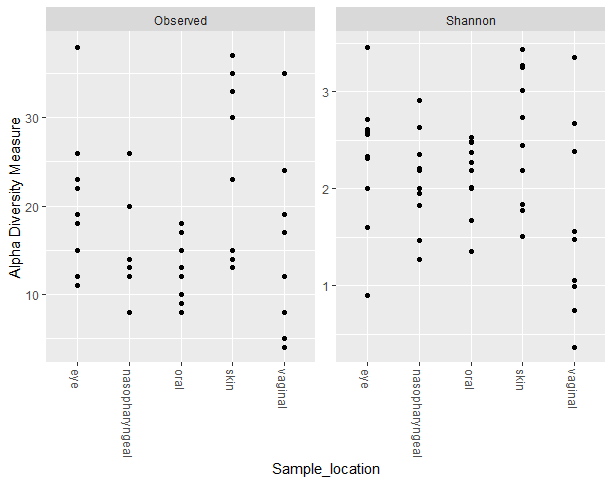
\includegraphics{/home/ray2g/Documents/Laboratory_Project_Final_Report/shannon_index.png}

\begin{figure}
\centering
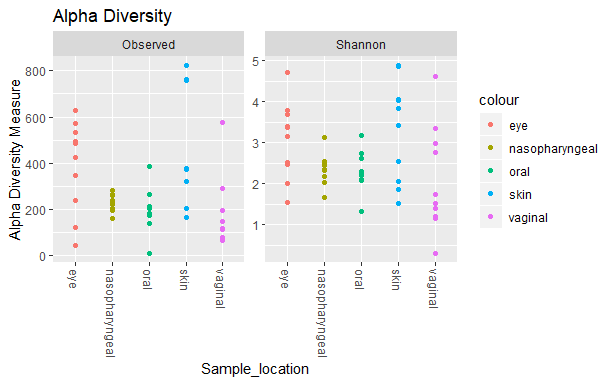
\includegraphics{/home/ray2g/Documents/Laboratory_Project_Final_Report/alpha_diversity.png}
\caption{alpha\_diversity}
\end{figure}

\hypertarget{beta-analysys-for-samples-location.}{%
\section{Beta Analysys for Samples
Location.}\label{beta-analysys-for-samples-location.}}

\begin{Shaded}
\begin{Highlighting}[]
\CommentTok{#Set the variables of the samples to use in the colors of the plots}
\NormalTok{Sample_location <-}\StringTok{ }\KeywordTok{factor}\NormalTok{(}\KeywordTok{sample_data}\NormalTok{(physeq2)}\OperatorTok{$}\NormalTok{Sample_location,}\DataTypeTok{levels =} \KeywordTok{c}\NormalTok{(}\StringTok{"eye"}\NormalTok{, }\StringTok{"nasopharyngeal"}\NormalTok{, }\StringTok{"oral"}\NormalTok{, }\StringTok{"skin"}\NormalTok{, }\StringTok{"vaginal"}\NormalTok{))}

\CommentTok{# Calculate bray-curtis distance for beta diversity}
\NormalTok{distbc <-}\StringTok{ }\KeywordTok{distance}\NormalTok{(physeq2, }\DataTypeTok{method =} \StringTok{"bray"}\NormalTok{)}
\NormalTok{ordBC <-}\StringTok{ }\KeywordTok{ordinate}\NormalTok{(}\DataTypeTok{physeq =}\NormalTok{ physeq2, }\DataTypeTok{method =} \StringTok{"PCoA"}\NormalTok{, }\DataTypeTok{distance =}\NormalTok{ distbc)}

\CommentTok{# Rarefation samples(optional)}
\NormalTok{ps.rarefied =}\StringTok{ }\KeywordTok{rarefy_even_depth}\NormalTok{(physeq2, }\DataTypeTok{rngseed=}\DecValTok{1}\NormalTok{, }\DataTypeTok{sample.size=}\FloatTok{0.9}\OperatorTok{*}\KeywordTok{min}\NormalTok{(}\KeywordTok{sample_sums}\NormalTok{(physeq2)), }\DataTypeTok{replace=}\NormalTok{F)}
\end{Highlighting}
\end{Shaded}

\begin{verbatim}
## `set.seed(1)` was used to initialize repeatable random subsampling.
\end{verbatim}

\begin{verbatim}
## Please record this for your records so others can reproduce.
\end{verbatim}

\begin{verbatim}
## Try `set.seed(1); .Random.seed` for the full vector
\end{verbatim}

\begin{verbatim}
## ...
\end{verbatim}

\begin{verbatim}
## 1444OTUs were removed because they are no longer 
## present in any sample after random subsampling
\end{verbatim}

\begin{verbatim}
## ...
\end{verbatim}

\begin{Shaded}
\begin{Highlighting}[]
\CommentTok{#Plot for beta diversity (with Bray-Curtis distance)}
\KeywordTok{plot_ordination}\NormalTok{(}\DataTypeTok{physeq =}\NormalTok{ physeq2,}\DataTypeTok{ordination =}\NormalTok{ ordBC,}\DataTypeTok{color =}\NormalTok{ Sample_location) }\OperatorTok{+}\StringTok{ }\KeywordTok{geom_point}\NormalTok{(}\KeywordTok{aes}\NormalTok{(}\DataTypeTok{color =}\NormalTok{ Sample_location), }\DataTypeTok{alpha =} \FloatTok{0.7}\NormalTok{, }\DataTypeTok{size =} \DecValTok{4}\NormalTok{)}
\end{Highlighting}
\end{Shaded}

\begin{verbatim}
## Warning in plot_ordination(physeq = physeq2, ordination = ordBC, color =
## Sample_location): The `color` variable argument should have length equal to
## 1.Taking first value.
\end{verbatim}

\begin{verbatim}
## Warning in plot_ordination(physeq = physeq2, ordination = ordBC, color =
## Sample_location): Color variable was not found in the available data you
## provided.No color mapped.
\end{verbatim}

\begin{verbatim}
## No available covariate data to map on the points for this plot `type`
\end{verbatim}

\includegraphics{Report_files/figure-latex/unnamed-chunk-7-1.pdf}

\begin{Shaded}
\begin{Highlighting}[]
\NormalTok{population_density <-}\StringTok{ }\KeywordTok{plot_landscape}\NormalTok{(ps.rarefied, }\StringTok{"NMDS"}\NormalTok{, }\StringTok{"bray"}\NormalTok{, }\DataTypeTok{col =} \StringTok{"Sample_location"}\NormalTok{) }\OperatorTok{+}\StringTok{ }\KeywordTok{labs}\NormalTok{(}\DataTypeTok{title =} \KeywordTok{paste}\NormalTok{(}\StringTok{"NMDS / Bray-Curtis"}\NormalTok{))}

\NormalTok{population_density }\OperatorTok{+}\StringTok{ }\KeywordTok{scale_color_brewer}\NormalTok{(}\DataTypeTok{palette=} \StringTok{"Dark2"}\NormalTok{) }\OperatorTok{+}\StringTok{ }\KeywordTok{scale_fill_gradient}\NormalTok{(}\DataTypeTok{low =} \StringTok{"#e0ecf4"}\NormalTok{, }\DataTypeTok{high =} \StringTok{"#6e016b"}\NormalTok{) }\OperatorTok{+}\StringTok{ }\KeywordTok{theme_classic}\NormalTok{()}
\end{Highlighting}
\end{Shaded}

\begin{verbatim}
## Scale for 'fill' is already present. Adding another scale for 'fill',
## which will replace the existing scale.
\end{verbatim}

\includegraphics{Report_files/figure-latex/unnamed-chunk-7-2.pdf}

\hypertarget{definitions-of-tops}{%
\section{Definitions of Tops}\label{definitions-of-tops}}

\begin{Shaded}
\begin{Highlighting}[]
\CommentTok{# Tops}

\NormalTok{top30<-}\StringTok{ }\KeywordTok{names}\NormalTok{(}\KeywordTok{sort}\NormalTok{(}\KeywordTok{taxa_sums}\NormalTok{(pseq), }\DataTypeTok{decreasing =} \OtherTok{TRUE}\NormalTok{))[}\DecValTok{1}\OperatorTok{:}\DecValTok{30}\NormalTok{]}
\NormalTok{pseq_top30 <-}\StringTok{ }\KeywordTok{transform_sample_counts}\NormalTok{(pseq, }\ControlFlowTok{function}\NormalTok{(OTU) OTU}\OperatorTok{/}\KeywordTok{sum}\NormalTok{(OTU))}
\NormalTok{pseq.top30 <-}\StringTok{ }\KeywordTok{prune_taxa}\NormalTok{(top30, pseq_top30)}

\NormalTok{top50<-}\StringTok{ }\KeywordTok{names}\NormalTok{(}\KeywordTok{sort}\NormalTok{(}\KeywordTok{taxa_sums}\NormalTok{(pseq), }\DataTypeTok{decreasing =} \OtherTok{TRUE}\NormalTok{))[}\DecValTok{1}\OperatorTok{:}\DecValTok{50}\NormalTok{]}
\NormalTok{pseq_top50 <-}\StringTok{ }\KeywordTok{transform_sample_counts}\NormalTok{(pseq, }\ControlFlowTok{function}\NormalTok{(OTU) OTU}\OperatorTok{/}\KeywordTok{sum}\NormalTok{(OTU))}
\NormalTok{pseq.top50 <-}\StringTok{ }\KeywordTok{prune_taxa}\NormalTok{(top50, pseq_top50)}

\NormalTok{top100<-}\StringTok{ }\KeywordTok{names}\NormalTok{(}\KeywordTok{sort}\NormalTok{(}\KeywordTok{taxa_sums}\NormalTok{(pseq), }\DataTypeTok{decreasing =} \OtherTok{TRUE}\NormalTok{))[}\DecValTok{1}\OperatorTok{:}\DecValTok{100}\NormalTok{]}
\NormalTok{pseq_top100 <-}\StringTok{ }\KeywordTok{transform_sample_counts}\NormalTok{(pseq, }\ControlFlowTok{function}\NormalTok{(OTU) OTU}\OperatorTok{/}\KeywordTok{sum}\NormalTok{(OTU))}
\NormalTok{pseq.top100 <-}\StringTok{ }\KeywordTok{prune_taxa}\NormalTok{(top100, pseq_top100)}

\CommentTok{# Head Taxa}

\KeywordTok{head}\NormalTok{(}\KeywordTok{get_taxa_unique}\NormalTok{(pseq.top20, }\StringTok{"Kingdom"}\NormalTok{))}
\end{Highlighting}
\end{Shaded}

\begin{verbatim}
## [1] "Bacteria"
\end{verbatim}

\begin{Shaded}
\begin{Highlighting}[]
\KeywordTok{head}\NormalTok{(}\KeywordTok{get_taxa_unique}\NormalTok{(pseq.top20, }\StringTok{"Phylum"}\NormalTok{))}
\end{Highlighting}
\end{Shaded}

\begin{verbatim}
## [1] "Firmicutes"     "Bacteroidetes"  "Actinobacteria" "Proteobacteria"
## [5] "Cyanobacteria"
\end{verbatim}

\begin{Shaded}
\begin{Highlighting}[]
\KeywordTok{head}\NormalTok{(}\KeywordTok{get_taxa_unique}\NormalTok{(pseq.top20, }\StringTok{"Class"}\NormalTok{))}
\end{Highlighting}
\end{Shaded}

\begin{verbatim}
## [1] "Clostridia"          "Bacteroidia"         "Actinobacteria"     
## [4] "Betaproteobacteria"  "Bacilli"             "Gammaproteobacteria"
\end{verbatim}

\begin{Shaded}
\begin{Highlighting}[]
\KeywordTok{head}\NormalTok{(}\KeywordTok{get_taxa_unique}\NormalTok{(pseq.top20, }\StringTok{"Order"}\NormalTok{))}
\end{Highlighting}
\end{Shaded}

\begin{verbatim}
## [1] "Clostridiales"   "Bacteroidales"   "Actinomycetales" "Neisseriales"   
## [5] "Bacillales"      "Pasteurellales"
\end{verbatim}

\begin{Shaded}
\begin{Highlighting}[]
\KeywordTok{head}\NormalTok{(}\KeywordTok{get_taxa_unique}\NormalTok{(pseq.top20, }\StringTok{"Family"}\NormalTok{))}
\end{Highlighting}
\end{Shaded}

\begin{verbatim}
## [1] "[Tissierellaceae]"  "Ruminococcaceae"    "Bacteroidaceae"    
## [4] "Corynebacteriaceae" "Micrococcaceae"     "Neisseriaceae"
\end{verbatim}

\begin{Shaded}
\begin{Highlighting}[]
\KeywordTok{head}\NormalTok{(}\KeywordTok{get_taxa_unique}\NormalTok{(pseq.top20, }\StringTok{"Genus"}\NormalTok{))}
\end{Highlighting}
\end{Shaded}

\begin{verbatim}
## [1] "Anaerococcus"    NA                "Bacteroides"     "Finegoldia"     
## [5] "Corynebacterium" "Rothia"
\end{verbatim}

\begin{Shaded}
\begin{Highlighting}[]
\KeywordTok{head}\NormalTok{(}\KeywordTok{get_taxa_unique}\NormalTok{(pseq.top20, }\StringTok{"Species"}\NormalTok{))}
\end{Highlighting}
\end{Shaded}

\begin{verbatim}
## [1] NA             "mucilaginosa" "copri"
\end{verbatim}

\hypertarget{creation-and-vizualization-of-barplots-for-each-location}{%
\section{Creation and Vizualization of barplots for each
location}\label{creation-and-vizualization-of-barplots-for-each-location}}

\begin{Shaded}
\begin{Highlighting}[]
\CommentTok{# BarPlot for each location}

\KeywordTok{plot_bar}\NormalTok{(pseq.top20, }\DataTypeTok{fill =} \StringTok{"Kingdom"}\NormalTok{) }\OperatorTok{+}\StringTok{ }\KeywordTok{facet_wrap}\NormalTok{(}\OperatorTok{~}\NormalTok{Sample_location, }\DataTypeTok{scales =} \StringTok{"free_x"}\NormalTok{, }\DataTypeTok{nrow =} \DecValTok{1}\NormalTok{)}
\end{Highlighting}
\end{Shaded}

\includegraphics{Report_files/figure-latex/unnamed-chunk-9-1.pdf}

\begin{Shaded}
\begin{Highlighting}[]
\KeywordTok{plot_bar}\NormalTok{(pseq.top20, }\DataTypeTok{fill =} \StringTok{"Phylum"}\NormalTok{) }\OperatorTok{+}\StringTok{ }\KeywordTok{facet_wrap}\NormalTok{(}\OperatorTok{~}\NormalTok{Sample_location, }\DataTypeTok{scales =} \StringTok{"free_x"}\NormalTok{, }\DataTypeTok{nrow =} \DecValTok{1}\NormalTok{)}
\end{Highlighting}
\end{Shaded}

\includegraphics{Report_files/figure-latex/unnamed-chunk-9-2.pdf}

\begin{Shaded}
\begin{Highlighting}[]
\KeywordTok{plot_bar}\NormalTok{(pseq.top20, }\DataTypeTok{fill =} \StringTok{"Class"}\NormalTok{) }\OperatorTok{+}\StringTok{ }\KeywordTok{facet_wrap}\NormalTok{(}\OperatorTok{~}\NormalTok{Sample_location, }\DataTypeTok{scales =} \StringTok{"free_x"}\NormalTok{, }\DataTypeTok{nrow =} \DecValTok{1}\NormalTok{)}
\end{Highlighting}
\end{Shaded}

\includegraphics{Report_files/figure-latex/unnamed-chunk-9-3.pdf}

\begin{Shaded}
\begin{Highlighting}[]
\KeywordTok{plot_bar}\NormalTok{(pseq.top20, }\DataTypeTok{fill =} \StringTok{"Order"}\NormalTok{) }\OperatorTok{+}\StringTok{ }\KeywordTok{facet_wrap}\NormalTok{(}\OperatorTok{~}\NormalTok{Sample_location, }\DataTypeTok{scales =} \StringTok{"free_x"}\NormalTok{, }\DataTypeTok{nrow =} \DecValTok{1}\NormalTok{)}
\end{Highlighting}
\end{Shaded}

\includegraphics{Report_files/figure-latex/unnamed-chunk-9-4.pdf}

\begin{Shaded}
\begin{Highlighting}[]
\KeywordTok{plot_bar}\NormalTok{(pseq.top20, }\DataTypeTok{fill =} \StringTok{"Family"}\NormalTok{) }\OperatorTok{+}\StringTok{ }\KeywordTok{facet_wrap}\NormalTok{(}\OperatorTok{~}\NormalTok{Sample_location, }\DataTypeTok{scales =} \StringTok{"free_x"}\NormalTok{, }\DataTypeTok{nrow =} \DecValTok{1}\NormalTok{)}
\end{Highlighting}
\end{Shaded}

\includegraphics{Report_files/figure-latex/unnamed-chunk-9-5.pdf}

\begin{Shaded}
\begin{Highlighting}[]
\KeywordTok{plot_bar}\NormalTok{(pseq.top20, }\DataTypeTok{fill =} \StringTok{"Genus"}\NormalTok{) }\OperatorTok{+}\StringTok{ }\KeywordTok{facet_wrap}\NormalTok{(}\OperatorTok{~}\NormalTok{Sample_location, }\DataTypeTok{scales =} \StringTok{"free_x"}\NormalTok{, }\DataTypeTok{nrow =} \DecValTok{1}\NormalTok{)}
\end{Highlighting}
\end{Shaded}

\includegraphics{Report_files/figure-latex/unnamed-chunk-9-6.pdf}

\begin{Shaded}
\begin{Highlighting}[]
\KeywordTok{plot_bar}\NormalTok{(pseq.top20, }\DataTypeTok{fill=} \StringTok{"Species"}\NormalTok{) }\OperatorTok{+}\StringTok{ }\KeywordTok{facet_wrap}\NormalTok{(}\OperatorTok{~}\NormalTok{Sample_location, }\DataTypeTok{scales =} \StringTok{"free_x"}\NormalTok{, }\DataTypeTok{nrow =} \DecValTok{1}\NormalTok{)}
\end{Highlighting}
\end{Shaded}

\includegraphics{Report_files/figure-latex/unnamed-chunk-9-7.pdf}

\hypertarget{creation-and-vizualization-of-barplots-for-all-the-samples-with-our-dataset-the-50-samples-one.}{%
\section{Creation and Vizualization of barplots for all the samples with
our dataset, the 50 samples
one.}\label{creation-and-vizualization-of-barplots-for-all-the-samples-with-our-dataset-the-50-samples-one.}}

\begin{Shaded}
\begin{Highlighting}[]
\CommentTok{# BarPlot }

\KeywordTok{plot_bar}\NormalTok{(pseq.top20, }\DataTypeTok{fill=}\StringTok{"Kingdom"}\NormalTok{)}
\end{Highlighting}
\end{Shaded}

\includegraphics{Report_files/figure-latex/unnamed-chunk-10-1.pdf}

\begin{Shaded}
\begin{Highlighting}[]
\KeywordTok{plot_bar}\NormalTok{(pseq.top20, }\DataTypeTok{fill=}\StringTok{"Phylum"}\NormalTok{)}
\end{Highlighting}
\end{Shaded}

\includegraphics{Report_files/figure-latex/unnamed-chunk-10-2.pdf}

\begin{Shaded}
\begin{Highlighting}[]
\KeywordTok{plot_bar}\NormalTok{(pseq.top20, }\DataTypeTok{fill=}\StringTok{"Class"}\NormalTok{)}
\end{Highlighting}
\end{Shaded}

\includegraphics{Report_files/figure-latex/unnamed-chunk-10-3.pdf}

\begin{Shaded}
\begin{Highlighting}[]
\KeywordTok{plot_bar}\NormalTok{(pseq.top20, }\DataTypeTok{fill=}\StringTok{"Order"}\NormalTok{)}
\end{Highlighting}
\end{Shaded}

\includegraphics{Report_files/figure-latex/unnamed-chunk-10-4.pdf}

\begin{Shaded}
\begin{Highlighting}[]
\KeywordTok{plot_bar}\NormalTok{(pseq.top20, }\DataTypeTok{fill=}\StringTok{"Family"}\NormalTok{)}
\end{Highlighting}
\end{Shaded}

\includegraphics{Report_files/figure-latex/unnamed-chunk-10-5.pdf}

\begin{Shaded}
\begin{Highlighting}[]
\KeywordTok{plot_bar}\NormalTok{(pseq.top20, }\DataTypeTok{fill=}\StringTok{"Genus"}\NormalTok{)}
\end{Highlighting}
\end{Shaded}

\includegraphics{Report_files/figure-latex/unnamed-chunk-10-6.pdf}

\begin{Shaded}
\begin{Highlighting}[]
\KeywordTok{plot_bar}\NormalTok{(pseq.top20, }\DataTypeTok{fill=}\StringTok{"Species"}\NormalTok{)}
\end{Highlighting}
\end{Shaded}

\includegraphics{Report_files/figure-latex/unnamed-chunk-10-7.pdf}

At the start of this analysis composition report we used the
plot\_composition function from microbiome package but beyond show the
otu names by ids, it dont assume the taxonomic level for each domain.

So i let them in the report to analyse which may not have worked
correctly.

Chatting in the forums it was said that

" The plot\_composition returns a ggplot object. My suggestion is to use
standard ggplot utilities for more fine-tuned figure manipulation. The
plot\_composition and other similar functions in the microbiome pkg are
designed to facilitate fast data exploration. Fine-tuning needs are so
variable and user dependent that it is not efficient to try to implement
most of those solutions in the function itself since manipulation tools
for ggplot objects exist already."

ggplot did not recognize the sample type provided so i dont proceed.

\begin{Shaded}
\begin{Highlighting}[]
\CommentTok{# Plot Composition for sample location}

\NormalTok{psl_composition_Kingdom <-}\StringTok{ }\KeywordTok{plot_composition}\NormalTok{(pseq.top20, }\DataTypeTok{taxonomic.level =} \StringTok{"Kingdom"}\NormalTok{, }\DataTypeTok{average_by =} \StringTok{"Sample_location"}\NormalTok{, }\DataTypeTok{transform =} \StringTok{"compositional"}\NormalTok{) }\OperatorTok{+}
\StringTok{  }\KeywordTok{labs}\NormalTok{(}\DataTypeTok{x =} \StringTok{"Sample Location"}\NormalTok{, }\DataTypeTok{y =} \StringTok{"Relative abundance (%)"}\NormalTok{, }\DataTypeTok{title =} \StringTok{"Relative abundance data"}\NormalTok{, }\DataTypeTok{subtitle =} \StringTok{"Kingdom"}\NormalTok{) }\OperatorTok{+}
\StringTok{  }\KeywordTok{geom_point}\NormalTok{(}\DataTypeTok{color=}\StringTok{"black"}\NormalTok{, }\DataTypeTok{position=}\StringTok{"jitter"}\NormalTok{, }\DataTypeTok{size=}\DecValTok{1}\NormalTok{) }\OperatorTok{+}\StringTok{ }\KeywordTok{theme_classic}\NormalTok{()}

\NormalTok{psl_composition_Phylum <-}\StringTok{ }\KeywordTok{plot_composition}\NormalTok{(pseq.top20, }\DataTypeTok{taxonomic.level =} \StringTok{"Phylum"}\NormalTok{, }\DataTypeTok{average_by =} \StringTok{"Sample_location"}\NormalTok{, }\DataTypeTok{transform =} \StringTok{"compositional"}\NormalTok{) }\OperatorTok{+}
\StringTok{  }\KeywordTok{labs}\NormalTok{(}\DataTypeTok{x =} \StringTok{"Sample Location"}\NormalTok{, }\DataTypeTok{y =} \StringTok{"Relative abundance (%)"}\NormalTok{, }\DataTypeTok{title =} \StringTok{"Relative abundance data"}\NormalTok{, }\DataTypeTok{subtitle =} \StringTok{"Phylum"}\NormalTok{) }\OperatorTok{+}
\StringTok{  }\KeywordTok{geom_point}\NormalTok{(}\DataTypeTok{color=}\StringTok{"black"}\NormalTok{, }\DataTypeTok{position=}\StringTok{"jitter"}\NormalTok{, }\DataTypeTok{size=}\DecValTok{1}\NormalTok{) }\OperatorTok{+}\StringTok{ }\KeywordTok{theme_classic}\NormalTok{()}

\NormalTok{psl_composition_Class <-}\StringTok{ }\KeywordTok{plot_composition}\NormalTok{(pseq.top20, }\DataTypeTok{taxonomic.level =} \StringTok{"Class"}\NormalTok{, }\DataTypeTok{average_by =} \StringTok{"Sample_location"}\NormalTok{, }\DataTypeTok{transform =} \StringTok{"compositional"}\NormalTok{) }\OperatorTok{+}
\StringTok{  }\KeywordTok{labs}\NormalTok{(}\DataTypeTok{x =} \StringTok{"Sample Location"}\NormalTok{, }\DataTypeTok{y =} \StringTok{"Relative abundance (%)"}\NormalTok{, }\DataTypeTok{title =} \StringTok{"Relative abundance data"}\NormalTok{, }\DataTypeTok{subtitle =} \StringTok{"Class"}\NormalTok{) }\OperatorTok{+}
\StringTok{  }\KeywordTok{geom_point}\NormalTok{(}\DataTypeTok{color=}\StringTok{"black"}\NormalTok{, }\DataTypeTok{position=}\StringTok{"jitter"}\NormalTok{, }\DataTypeTok{size=}\DecValTok{1}\NormalTok{) }\OperatorTok{+}\StringTok{ }\KeywordTok{theme_classic}\NormalTok{()}

\NormalTok{psl_composition_Order <-}\StringTok{ }\KeywordTok{plot_composition}\NormalTok{(pseq.top20, }\DataTypeTok{taxonomic.level =} \StringTok{"Order"}\NormalTok{, }\DataTypeTok{average_by =} \StringTok{"Sample_location"}\NormalTok{, }\DataTypeTok{transform =} \StringTok{"compositional"}\NormalTok{) }\OperatorTok{+}
\StringTok{  }\KeywordTok{labs}\NormalTok{(}\DataTypeTok{x =} \StringTok{"Sample Location"}\NormalTok{, }\DataTypeTok{y =} \StringTok{"Relative abundance (%)"}\NormalTok{, }\DataTypeTok{title =} \StringTok{"Relative abundance data"}\NormalTok{, }\DataTypeTok{subtitle =} \StringTok{"Order"}\NormalTok{) }\OperatorTok{+}
\StringTok{  }\KeywordTok{geom_point}\NormalTok{(}\DataTypeTok{color=}\StringTok{"black"}\NormalTok{, }\DataTypeTok{position=}\StringTok{"jitter"}\NormalTok{, }\DataTypeTok{size=}\DecValTok{1}\NormalTok{) }\OperatorTok{+}\StringTok{ }\KeywordTok{theme_classic}\NormalTok{()}

\NormalTok{psl_composition_Family <-}\StringTok{ }\KeywordTok{plot_composition}\NormalTok{(pseq.top20, }\DataTypeTok{taxonomic.level =} \StringTok{"Family"}\NormalTok{, }\DataTypeTok{average_by =} \StringTok{"Sample_location"}\NormalTok{, }\DataTypeTok{transform =} \StringTok{"compositional"}\NormalTok{) }\OperatorTok{+}
\StringTok{     }\KeywordTok{labs}\NormalTok{(}\DataTypeTok{x =} \StringTok{"Sample Location"}\NormalTok{, }\DataTypeTok{y =} \StringTok{"Relative abundance (%)"}\NormalTok{, }\DataTypeTok{title =} \StringTok{"Relative abundance data"}\NormalTok{, }\DataTypeTok{subtitle =} \StringTok{"Family"}\NormalTok{) }\OperatorTok{+}
\StringTok{     }\KeywordTok{geom_point}\NormalTok{(}\DataTypeTok{color=}\StringTok{"black"}\NormalTok{, }\DataTypeTok{position=}\StringTok{"jitter"}\NormalTok{, }\DataTypeTok{size=}\DecValTok{1}\NormalTok{) }\OperatorTok{+}\StringTok{ }\KeywordTok{theme_classic}\NormalTok{()}

\NormalTok{psl_composition_Genus <-}\StringTok{ }\KeywordTok{plot_composition}\NormalTok{(pseq.top20, }\DataTypeTok{taxonomic.level =} \StringTok{"genus"}\NormalTok{, }\DataTypeTok{average_by =} \StringTok{"Sample_location"}\NormalTok{, }\DataTypeTok{transform =} \StringTok{"compositional"}\NormalTok{) }\OperatorTok{+}
\StringTok{  }\KeywordTok{labs}\NormalTok{(}\DataTypeTok{x =} \StringTok{"Sample Location"}\NormalTok{, }\DataTypeTok{y =} \StringTok{"Relative abundance (%)"}\NormalTok{, }\DataTypeTok{title =} \StringTok{"Relative abundance data"}\NormalTok{, }\DataTypeTok{subtitle =} \StringTok{"Genus"}\NormalTok{) }\OperatorTok{+}
\StringTok{  }\KeywordTok{geom_point}\NormalTok{(}\DataTypeTok{color=}\StringTok{"black"}\NormalTok{, }\DataTypeTok{position=}\StringTok{"jitter"}\NormalTok{, }\DataTypeTok{size=}\DecValTok{1}\NormalTok{) }\OperatorTok{+}\StringTok{ }\KeywordTok{theme_classic}\NormalTok{()}

\NormalTok{psl_composition_Species <-}\StringTok{ }\KeywordTok{plot_composition}\NormalTok{(pseq.top20, }\DataTypeTok{taxonomic.level =} \StringTok{"genus"}\NormalTok{, }\DataTypeTok{average_by =} \StringTok{"Sample_location"}\NormalTok{, }\DataTypeTok{transform =} \StringTok{"compositional"}\NormalTok{) }\OperatorTok{+}
\StringTok{  }\KeywordTok{labs}\NormalTok{(}\DataTypeTok{x =} \StringTok{"Sample Location"}\NormalTok{, }\DataTypeTok{y =} \StringTok{"Relative abundance (%)"}\NormalTok{, }\DataTypeTok{title =} \StringTok{"Relative abundance data"}\NormalTok{, }\DataTypeTok{subtitle =} \StringTok{"Species"}\NormalTok{) }\OperatorTok{+}
\StringTok{  }\KeywordTok{geom_point}\NormalTok{(}\DataTypeTok{color=}\StringTok{"black"}\NormalTok{, }\DataTypeTok{position=}\StringTok{"jitter"}\NormalTok{, }\DataTypeTok{size=}\DecValTok{1}\NormalTok{) }\OperatorTok{+}\StringTok{ }\KeywordTok{theme_classic}\NormalTok{()}

\NormalTok{psl_composition_Kingdom}
\end{Highlighting}
\end{Shaded}

\includegraphics{Report_files/figure-latex/unnamed-chunk-11-1.pdf}

\begin{Shaded}
\begin{Highlighting}[]
\NormalTok{psl_composition_Phylum}
\end{Highlighting}
\end{Shaded}

\includegraphics{Report_files/figure-latex/unnamed-chunk-11-2.pdf}

\begin{Shaded}
\begin{Highlighting}[]
\NormalTok{psl_composition_Class}
\end{Highlighting}
\end{Shaded}

\includegraphics{Report_files/figure-latex/unnamed-chunk-11-3.pdf}

\begin{Shaded}
\begin{Highlighting}[]
\NormalTok{psl_composition_Order}
\end{Highlighting}
\end{Shaded}

\includegraphics{Report_files/figure-latex/unnamed-chunk-11-4.pdf}

\begin{Shaded}
\begin{Highlighting}[]
\NormalTok{psl_composition_Family}
\end{Highlighting}
\end{Shaded}

\includegraphics{Report_files/figure-latex/unnamed-chunk-11-5.pdf}

\begin{Shaded}
\begin{Highlighting}[]
\NormalTok{psl_composition_Genus}
\end{Highlighting}
\end{Shaded}

\includegraphics{Report_files/figure-latex/unnamed-chunk-11-6.pdf}

\begin{Shaded}
\begin{Highlighting}[]
\NormalTok{psl_composition_Species}
\end{Highlighting}
\end{Shaded}

\includegraphics{Report_files/figure-latex/unnamed-chunk-11-7.pdf}

\begin{Shaded}
\begin{Highlighting}[]
\CommentTok{# BarPlot}

\NormalTok{bp_Kingdom <-}\KeywordTok{plot_composition}\NormalTok{(pseq.top20,}
                             \DataTypeTok{taxonomic.level =} \StringTok{"Kigdom"}\NormalTok{, }\DataTypeTok{plot.type =} \StringTok{"barplot"}\NormalTok{) }\OperatorTok{+}\StringTok{ }
\StringTok{  }\KeywordTok{labs}\NormalTok{(}\DataTypeTok{x =} \StringTok{"Samples"}\NormalTok{, }\DataTypeTok{y =} \StringTok{"Relative abundance (%)"}\NormalTok{, }\DataTypeTok{title =} \StringTok{"Relative abundance data"}\NormalTok{, }\DataTypeTok{subtitle =} \StringTok{"Kingdom"}\NormalTok{) }\OperatorTok{+}\StringTok{ }
\StringTok{  }\KeywordTok{theme_ipsum}\NormalTok{(}\DataTypeTok{grid=}\StringTok{"Y"}\NormalTok{)}\OperatorTok{+}\StringTok{ }\KeywordTok{theme_grey}\NormalTok{() }\OperatorTok{+}\StringTok{ }\KeywordTok{theme}\NormalTok{(}\DataTypeTok{axis.text.x =} \KeywordTok{element_text}\NormalTok{(}\DataTypeTok{angle =} \DecValTok{90}\NormalTok{, }\DataTypeTok{hjust =} \DecValTok{1}\NormalTok{))}


\NormalTok{bp_Phylum <-}\KeywordTok{plot_composition}\NormalTok{(pseq.top20,}
                             \DataTypeTok{taxonomic.level =} \StringTok{"Phylum"}\NormalTok{, }\DataTypeTok{plot.type =} \StringTok{"barplot"}\NormalTok{) }\OperatorTok{+}
\StringTok{  }\KeywordTok{labs}\NormalTok{(}\DataTypeTok{x =} \StringTok{"Samples"}\NormalTok{, }\DataTypeTok{y =} \StringTok{"Relative abundance (%)"}\NormalTok{, }\DataTypeTok{title =} \StringTok{"Relative abundance data"}\NormalTok{, }\DataTypeTok{subtitle =} \StringTok{"Phylum"}\NormalTok{) }\OperatorTok{+}\StringTok{ }
\StringTok{  }\KeywordTok{theme_ipsum}\NormalTok{(}\DataTypeTok{grid=}\StringTok{"Y"}\NormalTok{) }\OperatorTok{+}\StringTok{ }\KeywordTok{theme_grey}\NormalTok{() }\OperatorTok{+}\StringTok{ }\KeywordTok{theme}\NormalTok{(}\DataTypeTok{axis.text.x =} \KeywordTok{element_text}\NormalTok{(}\DataTypeTok{angle =} \DecValTok{90}\NormalTok{, }\DataTypeTok{hjust =} \DecValTok{1}\NormalTok{))}


\NormalTok{bp_Class <-}\KeywordTok{plot_composition}\NormalTok{(pseq.top20,}
                             \DataTypeTok{taxonomic.level =} \StringTok{"Class"}\NormalTok{, }\DataTypeTok{plot.type =} \StringTok{"barplot"}\NormalTok{) }\OperatorTok{+}
\StringTok{  }\KeywordTok{labs}\NormalTok{(}\DataTypeTok{x =} \StringTok{"Samples"}\NormalTok{, }\DataTypeTok{y =} \StringTok{"Relative abundance (%)"}\NormalTok{, }\DataTypeTok{title =} \StringTok{"Relative abundance data"}\NormalTok{, }\DataTypeTok{subtitle =} \StringTok{"Class"}\NormalTok{) }\OperatorTok{+}\StringTok{ }
\StringTok{  }\KeywordTok{theme_ipsum}\NormalTok{(}\DataTypeTok{grid=}\StringTok{"Y"}\NormalTok{) }\OperatorTok{+}\StringTok{ }\KeywordTok{theme_grey}\NormalTok{() }\OperatorTok{+}\StringTok{ }\KeywordTok{theme}\NormalTok{(}\DataTypeTok{axis.text.x =} \KeywordTok{element_text}\NormalTok{(}\DataTypeTok{angle =} \DecValTok{90}\NormalTok{, }\DataTypeTok{hjust =} \DecValTok{1}\NormalTok{))}

\NormalTok{bp_Order <-}\KeywordTok{plot_composition}\NormalTok{(pseq.top20,}
                             \DataTypeTok{taxonomic.level =} \StringTok{"Order"}\NormalTok{, }\DataTypeTok{plot.type =} \StringTok{"barplot"}\NormalTok{) }\OperatorTok{+}
\StringTok{  }\KeywordTok{labs}\NormalTok{(}\DataTypeTok{x =} \StringTok{"Samples"}\NormalTok{, }\DataTypeTok{y =} \StringTok{"Relative abundance (%)"}\NormalTok{, }\DataTypeTok{title =} \StringTok{"Relative abundance data"}\NormalTok{, }\DataTypeTok{subtitle =} \StringTok{"Order"}\NormalTok{) }\OperatorTok{+}\StringTok{ }
\StringTok{  }\KeywordTok{theme_ipsum}\NormalTok{(}\DataTypeTok{grid=}\StringTok{"Y"}\NormalTok{)}\OperatorTok{+}\StringTok{ }\KeywordTok{theme_grey}\NormalTok{() }\OperatorTok{+}\StringTok{ }\KeywordTok{theme}\NormalTok{(}\DataTypeTok{axis.text.x =} \KeywordTok{element_text}\NormalTok{(}\DataTypeTok{angle =} \DecValTok{90}\NormalTok{, }\DataTypeTok{hjust =} \DecValTok{1}\NormalTok{))}


\NormalTok{bp_Family <-}\KeywordTok{plot_composition}\NormalTok{(pseq.top20,}
                             \DataTypeTok{taxonomic.level =} \StringTok{"Family"}\NormalTok{, }\DataTypeTok{plot.type =} \StringTok{"barplot"}\NormalTok{) }\OperatorTok{+}\StringTok{ }
\StringTok{                             }\KeywordTok{labs}\NormalTok{(}\DataTypeTok{x =} \StringTok{"Samples"}\NormalTok{, }\DataTypeTok{y =} \StringTok{"Relative abundance (%)"}\NormalTok{, }\DataTypeTok{title =} \StringTok{"Relative abundance data"}\NormalTok{, }\DataTypeTok{subtitle =} \StringTok{"Family"}\NormalTok{) }\OperatorTok{+}\StringTok{ }
\StringTok{                             }\KeywordTok{theme_ipsum}\NormalTok{(}\DataTypeTok{grid=}\StringTok{"Y"}\NormalTok{)}\OperatorTok{+}\StringTok{ }\KeywordTok{theme_grey}\NormalTok{() }\OperatorTok{+}\StringTok{ }\KeywordTok{theme}\NormalTok{(}\DataTypeTok{axis.text.x =} \KeywordTok{element_text}\NormalTok{(}\DataTypeTok{angle =} \DecValTok{90}\NormalTok{, }\DataTypeTok{hjust =} \DecValTok{1}\NormalTok{))}



\NormalTok{bp_Genus <-}\StringTok{ }\KeywordTok{plot_composition}\NormalTok{(pseq.top20,}
                      \DataTypeTok{taxonomic.level =} \StringTok{"Genus"}\NormalTok{, }\DataTypeTok{plot.type =} \StringTok{"barplot"}\NormalTok{) }\OperatorTok{+}
\StringTok{                      }\KeywordTok{labs}\NormalTok{(}\DataTypeTok{x =} \StringTok{"Samples"}\NormalTok{, }\DataTypeTok{y =} \StringTok{"Relative abundance (%)"}\NormalTok{, }\DataTypeTok{title =} \StringTok{"Relative abundance data"}\NormalTok{, }\DataTypeTok{subtitle =} \StringTok{"Genus"}\NormalTok{) }\OperatorTok{+}\StringTok{ }
\StringTok{                      }\KeywordTok{theme_ipsum}\NormalTok{(}\DataTypeTok{grid=}\StringTok{"Y"}\NormalTok{)}\OperatorTok{+}\StringTok{ }\KeywordTok{theme_grey}\NormalTok{() }\OperatorTok{+}\StringTok{ }\KeywordTok{theme}\NormalTok{(}\DataTypeTok{axis.text.x =} \KeywordTok{element_text}\NormalTok{(}\DataTypeTok{angle =} \DecValTok{90}\NormalTok{, }\DataTypeTok{hjust =} \DecValTok{1}\NormalTok{))}


\NormalTok{bp_Species <-}\StringTok{ }\KeywordTok{plot_composition}\NormalTok{(pseq.top20,}
                                \DataTypeTok{taxonomic.level =} \StringTok{"Species"}\NormalTok{, }\DataTypeTok{plot.type =} \StringTok{"barplot"}\NormalTok{) }\OperatorTok{+}\StringTok{ }
\StringTok{                                }\KeywordTok{labs}\NormalTok{(}\DataTypeTok{x =} \StringTok{"Samples"}\NormalTok{, }\DataTypeTok{y =} \StringTok{"Relative abundance (%)"}\NormalTok{, }\DataTypeTok{title =} \StringTok{"Relative abundance data"}\NormalTok{, }\DataTypeTok{subtitle =} \StringTok{"Species"}\NormalTok{) }\OperatorTok{+}\StringTok{ }
\StringTok{                                }\KeywordTok{theme_ipsum}\NormalTok{(}\DataTypeTok{grid=}\StringTok{"Y"}\NormalTok{)}\OperatorTok{+}\StringTok{ }\KeywordTok{theme_grey}\NormalTok{() }\OperatorTok{+}\StringTok{ }\KeywordTok{theme}\NormalTok{(}\DataTypeTok{axis.text.x =} \KeywordTok{element_text}\NormalTok{(}\DataTypeTok{angle =} \DecValTok{90}\NormalTok{, }\DataTypeTok{hjust =} \DecValTok{1}\NormalTok{))}

\NormalTok{bp_Kingdom}
\end{Highlighting}
\end{Shaded}

\includegraphics{Report_files/figure-latex/unnamed-chunk-12-1.pdf}

\begin{Shaded}
\begin{Highlighting}[]
\NormalTok{bp_Phylum}
\end{Highlighting}
\end{Shaded}

\includegraphics{Report_files/figure-latex/unnamed-chunk-12-2.pdf}

\begin{Shaded}
\begin{Highlighting}[]
\NormalTok{bp_Class}
\end{Highlighting}
\end{Shaded}

\includegraphics{Report_files/figure-latex/unnamed-chunk-12-3.pdf}

\begin{Shaded}
\begin{Highlighting}[]
\NormalTok{bp_Order}
\end{Highlighting}
\end{Shaded}

\includegraphics{Report_files/figure-latex/unnamed-chunk-12-4.pdf}

\begin{Shaded}
\begin{Highlighting}[]
\NormalTok{bp_Family}
\end{Highlighting}
\end{Shaded}

\includegraphics{Report_files/figure-latex/unnamed-chunk-12-5.pdf}

\begin{Shaded}
\begin{Highlighting}[]
\NormalTok{bp_Genus}
\end{Highlighting}
\end{Shaded}

\includegraphics{Report_files/figure-latex/unnamed-chunk-12-6.pdf}

\begin{Shaded}
\begin{Highlighting}[]
\NormalTok{bp_Species}
\end{Highlighting}
\end{Shaded}

\includegraphics{Report_files/figure-latex/unnamed-chunk-12-7.pdf}

\hypertarget{heatmaps}{%
\section{HeatMaps}\label{heatmaps}}

\begin{Shaded}
\begin{Highlighting}[]
\CommentTok{# Heatmap}

\CommentTok{#k_bacteria <- subset_taxa(pseq, Kingdom =="Bacteria")}
\CommentTok{#heatmap(otu_table(k_bacteria), scale="column", col = terrain.colors(256), main="Heatmap | Kingdom |Bacteria")}

\CommentTok{# Agregate by Domain}
\NormalTok{pseq_kingdom <-}\StringTok{ }\KeywordTok{aggregate_taxa}\NormalTok{(pseq, }\StringTok{"Kingdom"}\NormalTok{)}
\NormalTok{pseq_phylum <-}\StringTok{ }\KeywordTok{aggregate_taxa}\NormalTok{(pseq, }\StringTok{"Phylum"}\NormalTok{)}
\NormalTok{pseq_class <-}\StringTok{ }\KeywordTok{aggregate_taxa}\NormalTok{(pseq, }\StringTok{"Class"}\NormalTok{)}
\NormalTok{pseq_order <-}\StringTok{ }\KeywordTok{aggregate_taxa}\NormalTok{(pseq, }\StringTok{"Order"}\NormalTok{)}
\NormalTok{pseq_family <-}\StringTok{ }\KeywordTok{aggregate_taxa}\NormalTok{(pseq, }\StringTok{"Family"}\NormalTok{) }
\NormalTok{pseq_genus <-}\StringTok{ }\KeywordTok{aggregate_taxa}\NormalTok{(pseq, }\StringTok{"Genus"}\NormalTok{)}
\NormalTok{pseq_Species <-}\StringTok{ }\KeywordTok{aggregate_taxa}\NormalTok{(pseq, }\StringTok{"Species"}\NormalTok{)}

\KeywordTok{plot_heatmap}\NormalTok{(pseq_kingdom, }\DataTypeTok{taxa.label=}\StringTok{"Kingdom"}\NormalTok{, }\DataTypeTok{title =} \StringTok{" HeatMap | Kingdom"}\NormalTok{)}
\end{Highlighting}
\end{Shaded}

\begin{verbatim}
## Warning in metaMDS(veganifyOTU(physeq), distance, ...): stress is (nearly)
## zero: you may have insufficient data
\end{verbatim}

\begin{verbatim}
## Warning: Transformation introduced infinite values in discrete y-axis
\end{verbatim}

\includegraphics{Report_files/figure-latex/unnamed-chunk-13-1.pdf}

\begin{Shaded}
\begin{Highlighting}[]
\KeywordTok{plot_heatmap}\NormalTok{(pseq_phylum, }\DataTypeTok{taxa.label=}\StringTok{"Phylum"}\NormalTok{, }\DataTypeTok{title =} \StringTok{" HeatMap | Phylum"}\NormalTok{)}
\end{Highlighting}
\end{Shaded}

\begin{verbatim}
## Warning: Transformation introduced infinite values in discrete y-axis
\end{verbatim}

\includegraphics{Report_files/figure-latex/unnamed-chunk-13-2.pdf}

\begin{Shaded}
\begin{Highlighting}[]
\KeywordTok{plot_heatmap}\NormalTok{(pseq_class, }\DataTypeTok{taxa.label=}\StringTok{"Class"}\NormalTok{, }\DataTypeTok{title =} \StringTok{" HeatMap | Class"}\NormalTok{)}
\end{Highlighting}
\end{Shaded}

\begin{verbatim}
## Warning: Transformation introduced infinite values in discrete y-axis
\end{verbatim}

\includegraphics{Report_files/figure-latex/unnamed-chunk-13-3.pdf}

\begin{Shaded}
\begin{Highlighting}[]
\KeywordTok{plot_heatmap}\NormalTok{(pseq_order, }\DataTypeTok{taxa.label=}\StringTok{"Order"}\NormalTok{, }\DataTypeTok{title =} \StringTok{" HeatMap | Order"}\NormalTok{)}
\end{Highlighting}
\end{Shaded}

\begin{verbatim}
## Warning: Transformation introduced infinite values in discrete y-axis
\end{verbatim}

\includegraphics{Report_files/figure-latex/unnamed-chunk-13-4.pdf}

\begin{Shaded}
\begin{Highlighting}[]
\KeywordTok{plot_heatmap}\NormalTok{(pseq_family, }\DataTypeTok{taxa.label=}\StringTok{"Family"}\NormalTok{, }\DataTypeTok{title =} \StringTok{" HeatMap | Family"}\NormalTok{)}
\end{Highlighting}
\end{Shaded}

\begin{verbatim}
## Warning: Transformation introduced infinite values in discrete y-axis
\end{verbatim}

\includegraphics{Report_files/figure-latex/unnamed-chunk-13-5.pdf}

\begin{Shaded}
\begin{Highlighting}[]
\KeywordTok{plot_heatmap}\NormalTok{(pseq_genus, }\DataTypeTok{taxa.label=}\StringTok{"Genus"}\NormalTok{, }\DataTypeTok{title =} \StringTok{" HeatMap | Genus"}\NormalTok{)}
\end{Highlighting}
\end{Shaded}

\begin{verbatim}
## Warning: Transformation introduced infinite values in discrete y-axis
\end{verbatim}

\includegraphics{Report_files/figure-latex/unnamed-chunk-13-6.pdf}

\begin{Shaded}
\begin{Highlighting}[]
\KeywordTok{plot_heatmap}\NormalTok{(pseq_Species, }\DataTypeTok{taxa.label=}\StringTok{"Species"}\NormalTok{, }\DataTypeTok{title =} \StringTok{" HeatMap | Species"}\NormalTok{)}
\end{Highlighting}
\end{Shaded}

\begin{verbatim}
## Warning: Transformation introduced infinite values in discrete y-axis
\end{verbatim}

\includegraphics{Report_files/figure-latex/unnamed-chunk-13-7.pdf}

\hypertarget{session-info}{%
\section{Session Info}\label{session-info}}

\begin{Shaded}
\begin{Highlighting}[]
\KeywordTok{sessionInfo}\NormalTok{()}
\end{Highlighting}
\end{Shaded}

\begin{verbatim}
## R version 3.5.1 (2018-07-02)
## Platform: x86_64-pc-linux-gnu (64-bit)
## Running under: Ubuntu 18.04.1 LTS
## 
## Matrix products: default
## BLAS: /home/ray2g/miniconda3/envs/rstudio/lib/R/lib/libRblas.so
## LAPACK: /home/ray2g/miniconda3/envs/rstudio/lib/R/lib/libRlapack.so
## 
## locale:
##  [1] LC_CTYPE=en_US.UTF-8       LC_NUMERIC=C              
##  [3] LC_TIME=en_US.UTF-8        LC_COLLATE=en_US.UTF-8    
##  [5] LC_MONETARY=en_US.UTF-8    LC_MESSAGES=en_US.UTF-8   
##  [7] LC_PAPER=en_US.UTF-8       LC_NAME=C                 
##  [9] LC_ADDRESS=C               LC_TELEPHONE=C            
## [11] LC_MEASUREMENT=en_US.UTF-8 LC_IDENTIFICATION=C       
## 
## attached base packages:
## [1] stats     graphics  grDevices utils     datasets  methods   base     
## 
## other attached packages:
## [1] bindrcpp_0.2.2     ape_5.2            tinytex_0.9       
## [4] RColorBrewer_1.1-2 microbiome_1.2.1   hrbrthemes_0.5.0.1
## [7] ggplot2_3.1.0      phyloseq_1.24.2    biomformat_1.8.0  
## 
## loaded via a namespace (and not attached):
##  [1] Rcpp_0.12.19        lattice_0.20-35     tidyr_0.8.1        
##  [4] Biostrings_2.48.0   assertthat_0.2.0    digest_0.6.18      
##  [7] foreach_1.4.4       R6_2.3.0            plyr_1.8.4         
## [10] stats4_3.5.1        evaluate_0.12       pillar_1.3.0       
## [13] zlibbioc_1.26.0     rlang_0.2.2         lazyeval_0.2.1     
## [16] data.table_1.11.8   extrafontdb_1.0     vegan_2.5-2        
## [19] S4Vectors_0.18.3    Matrix_1.2-14       rmarkdown_1.11     
## [22] labeling_0.3        splines_3.5.1       extrafont_0.17     
## [25] stringr_1.3.1       igraph_1.2.2        munsell_0.5.0      
## [28] compiler_3.5.1      xfun_0.4            pkgconfig_2.0.2    
## [31] BiocGenerics_0.26.0 multtest_2.36.0     mgcv_1.8-24        
## [34] htmltools_0.3.6     tidyselect_0.2.5    tibble_1.4.2       
## [37] IRanges_2.14.12     codetools_0.2-15    permute_0.9-4      
## [40] crayon_1.3.4        dplyr_0.7.7         withr_2.1.2        
## [43] MASS_7.3-51         grid_3.5.1          nlme_3.1-137       
## [46] jsonlite_1.5        Rttf2pt1_1.3.7      gtable_0.2.0       
## [49] magrittr_1.5        scales_1.0.0        stringi_1.2.4      
## [52] XVector_0.20.0      reshape2_1.4.3      Rhdf5lib_1.2.1     
## [55] iterators_1.0.10    tools_3.5.1         ade4_1.7-13        
## [58] Biobase_2.40.0      glue_1.3.0          purrr_0.2.5        
## [61] parallel_3.5.1      survival_2.42-6     yaml_2.2.0         
## [64] colorspace_1.3-2    rhdf5_2.24.0        cluster_2.0.7-1    
## [67] knitr_1.21          bindr_0.1.1
\end{verbatim}


\end{document}
